\documentclass[11pt]{standalone}
\usepackage{amssymb}
\usepackage{amsmath}
\usepackage[no-math]{fontspec}
\usepackage{unicode-math}
\usepackage{libertinus}
\usepackage{pgf,xcolor}
\usepackage{tikz}
\usetikzlibrary{arrows.meta, backgrounds}
\usepackage{pgfplots}
\pgfplotsset{compat=newest}

\definecolor{my_darkgray}{HTML}{484949}
\definecolor{my_lightgray}{HTML}{F3F4F4}
\definecolor{my_darkblue}{HTML}{005A94}
\definecolor{my_lightblue}{HTML}{CCDEE9}
\definecolor{my_yellow}{HTML}{FFEC7F}
\definecolor{my_red}{HTML}{E60000}
\definecolor{my_orange}{HTML}{E87846}

\begin{document}
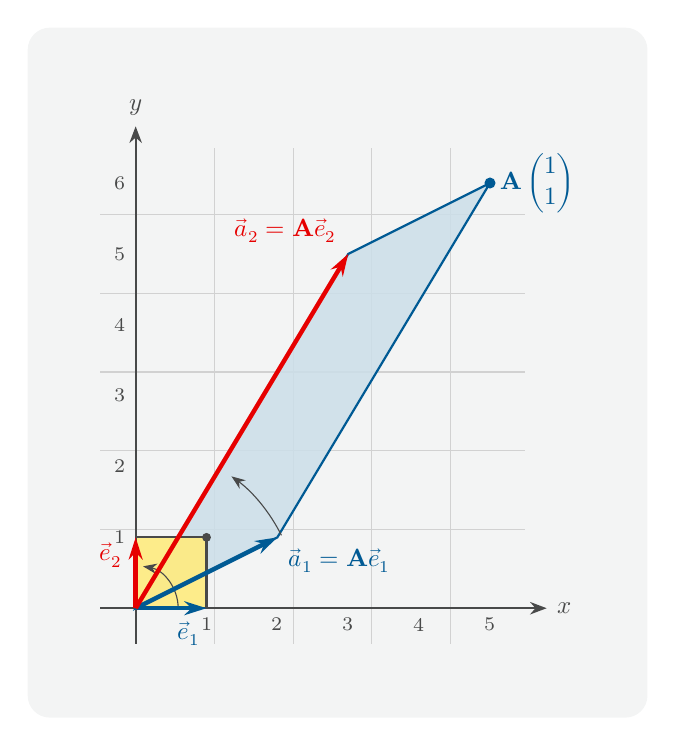
\begin{tikzpicture}[
    show background rectangle,
    background rectangle/.style={fill=my_lightgray, rounded corners=8pt},
    inner frame sep=0.8cm,
    x=0.9cm, y=0.9cm,
    vec/.style={-{Stealth[length=8pt, width=5pt]}, ultra thick}
]

% ---------------------------------------------------------------
%  Einheitsquadrat und sein Bild unter A = (2 3; 1 5):
%    e1 -> a1 = (2, 1),  e2 -> a2 = (3, 5),  e1 + e2 -> (5, 6)
% ---------------------------------------------------------------

% Gitter und Achsen
\draw[my_darkgray!25, thin] (-0.5, -0.5) grid (5.5, 6.5);
\draw[-{Stealth[length=6pt]}, thick, my_darkgray] (-0.5, 0) -- (5.8, 0)
    node[right, font=\small] {$x$};
\draw[-{Stealth[length=6pt]}, thick, my_darkgray] (0, -0.5) -- (0, 6.8)
    node[above, font=\small] {$y$};
\foreach \x in {1, ..., 5}
    \node[below, font=\scriptsize, my_darkgray] at (\x, 0) {$\x$};
\foreach \y in {1, ..., 6}
    \node[left, font=\scriptsize, my_darkgray] at (0, \y) {$\y$};

% Bild: Parallelogramm
\fill[my_lightblue, opacity=0.85] (0, 0) -- (2, 1) -- (5, 6) -- (3, 5) -- cycle;
\draw[my_darkblue, thick] (0, 0) -- (2, 1) -- (5, 6) -- (3, 5) -- cycle;

% Urbild: Einheitsquadrat
\fill[my_yellow, opacity=0.9] (0, 0) rectangle (1, 1);
\draw[my_darkgray, thick] (0, 0) rectangle (1, 1);

% Orientierungsboegen
\draw[my_darkgray, -{Stealth[length=5pt]}] (0:0.6) arc[start angle=0, end angle=80, radius=0.6];
\draw[my_darkgray, -{Stealth[length=5pt]}] (26.57:2.3) arc[start angle=26.57, end angle=54, radius=2.3];

% Einheitsvektoren
\draw[vec, my_darkblue] (0, 0) -- (1, 0);
\draw[vec, my_red] (0, 0) -- (0, 1);
\node[below, font=\small, my_darkblue] at (0.75, -0.05) {$\vec{e}_1$};
\node[left, font=\small, my_red] at (-0.05, 0.75) {$\vec{e}_2$};

% Bildvektoren
\draw[vec, my_darkblue] (0, 0) -- (2, 1)
    node[below right, font=\small] {$\vec{a}_1 = \mathbf{A}\vec{e}_1$};
\draw[vec, my_red] (0, 0) -- (3, 5)
    node[above left, font=\small] {$\vec{a}_2 = \mathbf{A}\vec{e}_2$};

% Ecke e1 + e2 und ihr Bild
\fill[my_darkgray] (1, 1) circle (1.6pt);
\fill[my_darkblue] (5, 6) circle (2pt)
    node[right, font=\small] {$\mathbf{A}\begin{pmatrix} 1 \\ 1 \end{pmatrix}$};

\end{tikzpicture}
\end{document}
